%Caso de uso 5
\begin{UseCase} {CU1.1.5}{Cobrar}{
	El empleado confirmará la venta, agregará el pago realizado por el cliente y generará el ticket de compra.
}

\UCitem{Versión}{1.0}
\UCccsection{Administración}
\UCccitem{Autor}{Lechuga Canales Héctor Jair}
\UCccitem{Evaluador}{Luis enrique Vázquez}
\UCccitem{Operación}{Ventas}
\UCccitem{Prioridad}{Alta}
\UCccitem{Complejidad}{Media}
\UCccitem{Volatilidad}{Baja}
\UCccitem{Madurez}{Alta}
\UCccitem{Estatus}{Edición}
\UCccitem{Fecha del último estatus}{02 de enero}

% Copie y pegue este bloque tantas veces como revisiones tenga el caso de uso.
% Esta sección la debe llenar solo el Revisor
% --------------------------------------------------------

% Revisión Versión 
% Anote la versión que se revisó
\UCccsection{Revisión Versión 0.1 }

% Fecha
% Anote la fecha en que se terminó la revisión
\UCccitem{Fecha}{03 de enero} 

% Evaluador
% Coloque el nombre completo de quien realizó la revisión
\UCccitem{Evaluador}{Luis enrique Vázquez}

% Resultado
% Coloque la palabra que mas se apegue al tipo de acción que el analista debe realizar
\UCccitem{Resultado}{redacción y ortografía}

% Observaciones
% Liste los cambios que debe realizar el Analista.
\UCccitem{Observaciones}{acentos y signos de puntuación}

% --------------------------------------------------------
	
\UCsection{Atributos}
	\UCitem{Actor(es)}
	{
		\cdtRef{Actor:RT}{Vendedor}
	}
	\UCitem{Propósito}
	{
		Confirmar la venta y generar el ticket.
	}
	\UCitem{Entradas}
	{
		
		\UCli Cantidad de dinero entregada por el cliente.
	}
	\UCitem{Salidas}
	{
		\UCli Código de barras 
		\UCli Descripción del producto
		\UCli Precio de venta
		\UCli Piezas
		\UCli Existencia actual
		\UCli Total a pagar
		\UCli Ticket de la compra
	}

	\UCitem{Precondiciones}
	{
		\UCli Debe estar agregado mínimo un producto dentro del carrito de compras.

	}
	\UCitem{Postcondiciones}
	{
		El sistema debe actualizar la BD de productos e historial de ventas.
	}
	\UCitem{Reglas de negocio}
	{
		ninguna
	}
	\UCitem{Errores}
	{
		Ninguna
	}
	\UCitem{Tipo}{}
\end{UseCase}

%Trayectoria principal

\begin{UCtrayectoria}
		
	\UCpaso [\UCactor]Selecciona el botón \cdtButton{Cobrar} ubicado en la interfaz carrito. consultar en página \pageref{UI: carrito}
	\UCpaso [\UCsist]Muestra una pantalla emergente llamada 'cobrar' consultar en página \pageref{UI: carrito Cobrar} con un text "cantidad a pagar" seguido del importe total de la compra y otro text "cantidad recibida" seguido de un input text donde se agregará la cantudad de efectivo recibida.
	\UCpaso [\UCactor]Ingresa la cantidad que le pagaron.
	\UCpaso [\UCactor]Selecciona el botón \cdtButton{confirmar}. \refTray{A}
	\UCpaso [\UCsist] En una pantalla mergente llamada 'Ticket' consultar en página \pageref{UI: carrito ticket}, genera una vista previa del ticket con todos los artículos comprados y datos de la farmacia.
	\UCpaso [\UCsist]Muestra la cantidad del vuelto en la parte inferior de la pantalla 'Ticket'.consultar en página \pageref{UI: carrito ticket}
	\UCpaso [\UCactor] Selecciona el botón \cdtButton{Confirmar}
	\UCpaso [\UCsist]Guarda el ticket en el historial de ventas 
	\UCpaso [\UCsist]Imprime el ticket para el cliente.
	\UCpaso [\UCsist]Guarda los cambios necesarios dentro de la BD de inventario.
	\UCpaso [\UCsist]Regresa a la pantalla 'carrito' para registrar una nueva venta. consultar en página \pageref{UI: carrito}
\end{UCtrayectoria}


% Trayectorias alternativas
Trayectoria alternativa A

\begin{UCtrayectoriaA}{A}{El cleinte desea eliminar productos o la venta total}

	\UCpaso [\UCactor] Selecciona boton \cdtButton{Cancelar} dentro de la pantalla "cobrar".  consultar en página \pageref{UI: carrito Cobrar} 	
	\UCpaso [\UCsist]Regresamos al paso \ref{CU 1.1.4:P1} de la TP.
\end{UCtrayectoriaA}


{
\begin{flushleft}
	% Clases
	\newpage
	\Large{Clases}\\
	\rule{14cm}{0.5pt}

	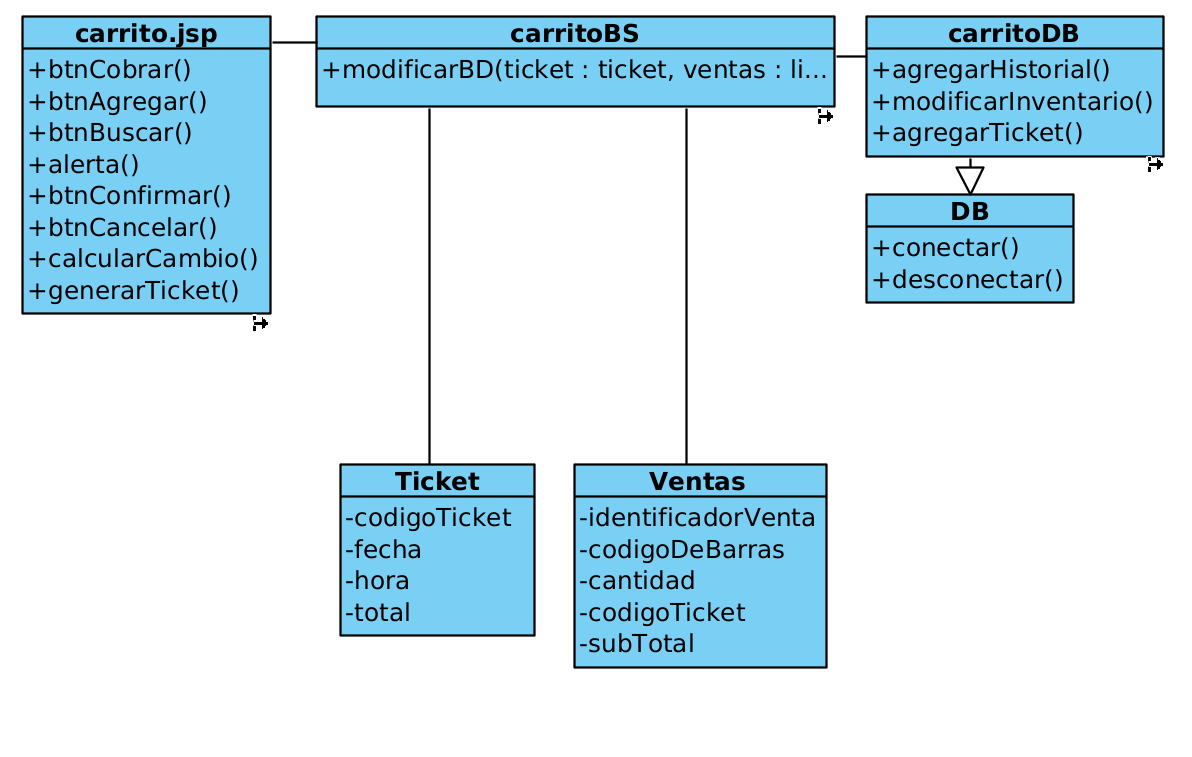
\includegraphics[width=14cm]{casouso/cu1.1.5/images/clases.png}\\	

	% Secuencia
	\newpage
	\Large{Secuencia}\\
	\rule{14cm}{0.5pt}

	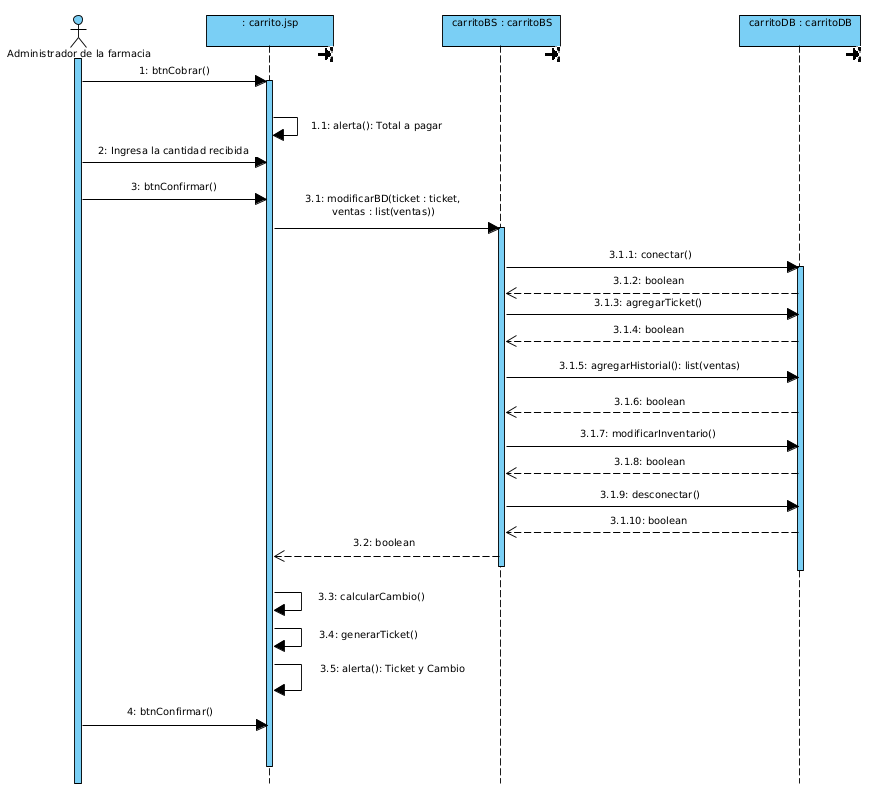
\includegraphics[width=14cm]{casouso/cu1.1.5/images/secuencias.png}\\	
	
\end{flushleft}
}